\documentclass[12pt]{article}
\usepackage{graphicx} % Required for inserting images
\usepackage[margin=0.5in]{geometry}
\usepackage{amsmath, amssymb}
\usepackage{mathrsfs}

\title{E\&M Equations}
\author{Gabriel Decker, A02308593}

\usepackage{soul}


% Dr. David Brown Commands
\newcommand{\ds}{\displaystyle}
\newcommand{\R}{\mathbb{R}}
\newcommand{\N}{\mathbb{N}}
\newcommand{\Q}{\mathbb{Q}}
\newcommand{\C}{\mathbb{C}}


% Commands to get script r
\usepackage{calligra}
\DeclareMathAlphabet{\mathcalligra}{T1}{calligra}{m}{n}
\DeclareFontShape{T1}{calligra}{m}{n}{<->s*[2.2]callig15}{}
\newcommand{\scripty}[1]{\ensuremath{\mathcalligra{#1}}}

% Unit commands
\newcommand{\degree}{\text{°}}
\newcommand{\unitSpeed}{\frac{\text{m}}{\text{s}}}
\newcommand{\unitAcceleration}{\frac{\text{m}}{\text{s}^2}}

% Constant commands
\newcommand{\avogadro}{6.022\times10^{23}}

\newcommand{\boltzmannConstK}{1.381\times10^{-23}\frac{\text{J}}{\text{K}}}
\newcommand{\planckConst}{6.626\times10^{-34}\text{J}\cdot\text{s}}

\newcommand{\atmP}{1.01325\times10^5\,\text{Pa}}

\begin{document}

\maketitle
\begin{flushleft}


\textbf{Math Facts}\\~\\
Law of cosines: $\ds C^2=A^2+B^2-2AB\cos(c)$\\~\\

\textbf{Shape facts}\\~\\
\textit{Circle}\\
Area: $\pi r^2$\\
Circumference: $2\pi r$\\~\\

\textit{Cylinder}\\
Volume: $\pi r^2h$\\
Surface Area: $\pi r^2+\pi r^2+2\pi rh$\\~\\

\textit{Sphere}\\
Volume: $\frac{4}{3}\pi r^3$\\
Surface Area: $4\pi r^2$\\~\\~\\

\textbf{Vectors}\\
$\hat{r}=\vec{r}/r$\\
$||\vec{a}+\vec{b}||^2=a^2+b^2+2\vec{a}\cdot\vec{b}$\\
Spherical to Cartesian Position: $\vec{r}=\rho(\sin(\theta)\cos(\phi)\hat{x}+\sin(\theta)\sin(\phi)\hat{y}+\cos(\theta)\hat{z})$\\
Cross products: $\hat{x}\times\hat{y}=\hat{z}$, $\hat{y}\times\hat{z}=\hat{x}$, $\hat{z}\times\hat{x}=\hat{y}$\\~\\

\textbf{Coordinate Conversions}\\
\textit{Cylindrical}\\
$x=s\cos(\phi)$, $y=s\sin(\phi)$, $z=z$\\
$s=\sqrt{x^2+y^2}$, $\phi=\arctan(\frac{y}{x})\ (x>0)$\\~\\

\textit{Spherical}\\
$x=r\sin(\theta)\cos(\phi)$, $y=r\sin(\theta)\sin(\phi)$, $z=r\cos(\theta)$\\
$r=\sqrt{x^2+y^2+z^2}$\\~\\


\textbf{Differential Calculus}\\~\\
\textit{Cartesian Coordinates}\\~\\

$\ds dT(x,y,z)=\frac{\partial T}{\partial x}dx+\frac{\partial T}{\partial y}dy+\frac{\partial T}{\partial z}dz$\\
$\ds \nabla=\frac{\partial}{\partial x}\hat{x}+\frac{\partial}{\partial y}\hat{y}+\frac{\partial}{\partial z}\hat{z}$\\
$\ds \nabla V(x,y,z)=\frac{\partial V}{\partial x}\hat{x}+\frac{\partial V}{\partial y}\hat{y}+\frac{\partial V}{\partial z}\hat{z}$\\
$\ds \vec{\nabla}\cdot\vec{E}=\frac{\partial E_x}{\partial x}+\frac{\partial E_y}{\partial y}+\frac{\partial E_z}{\partial z}$\\
$\ds \vec{\nabla}\times\vec{E}=\hat{x}(\frac{\partial E_z}{\partial y}-\frac{\partial E_y}{\partial z})+\hat{y}(\frac{\partial E_x}{\partial z}-\frac{\partial E_z}{\partial x})+\hat{z}(\frac{\partial E_y}{\partial x}-\frac{\partial E_x}{\partial y})$\\
$\ds\vec{\nabla}\cdot(\nabla V)=\nabla^2V=\frac{\partial^2 V}{\partial x^2}+\frac{\partial^2 V}{\partial y^2}+\frac{\partial^2 V}{\partial z^2}$\\~\\

\textit{Spherical Coordinates}\\~\\
$\ds \nabla=\frac{\partial}{\partial r}\hat{r}+\frac{1}{r}\frac{\partial}{\partial\theta}\hat{\theta}+\frac{1}{r\sin(\theta)}\frac{\partial}{\partial\phi}\hat{\phi}$\\
$\ds \nabla V(r,\theta,\phi)=\frac{\partial V}{\partial r}\hat{r}+\frac{1}{r}\frac{\partial V}{\partial\theta}\hat{\theta}+\frac{1}{r\sin(\theta)}\frac{\partial V}{\partial\phi}\hat{\phi}$\\
$\ds \vec{\nabla}\cdot \vec{E}=\frac{1}{r^2}\frac{\partial }{\partial r}(r^2E_r)+\frac{1}{r\sin(\theta)}\frac{\partial }{\partial\theta}(\sin(\theta)E_\theta)+\frac{1}{r\sin(\theta)}\frac{\partial E_\phi}{\partial\phi}$\\
$\ds \vec{\nabla}\times\vec{E}=\frac{1}{r\sin(\theta)}\left[\frac{\partial}{\partial \theta}(\sin(\theta)E_\phi)-\frac{\partial E_\theta}{\partial \phi}\right]\hat{r}+\frac{1}{r}\left[\frac{1}{\sin(\theta)}\frac{\partial E_r}{\partial \phi}-\frac{\partial}{\partial r}(rE_\phi)\right]\hat{\theta}+\frac{1}{r}\left[\frac{\partial}{\partial r}(rE_\theta)-\frac{\partial E_r}{\partial \theta}\right]\hat{\phi}$\\
$\ds \vec{\nabla}\cdot(\nabla V)=\nabla^2V=\frac{1}{r^2}\frac{\partial}{\partial r}\left(r^2\frac{\partial V}{\partial r}\right)+\frac{1}{r^2\sin(\theta)}\frac{\partial}{\partial \theta}\left(\sin(\theta)\frac{\partial V}{\partial \theta}\right)+\frac{1}{r^2\sin^2(\theta)}\frac{\partial^2 V}{\partial \phi^2}$\\~\\

\textit{Cylindrical Coordinates}\\~\\
$\ds \nabla=\frac{\partial}{\partial s}\hat{s}+\frac{1}{s}\frac{\partial}{\partial\phi}\hat{\phi}+\frac{\partial}{\partial z}\hat{z}$\\
$\ds \nabla V=\frac{\partial V}{\partial s}\hat{s}+\frac{1}{s}\frac{\partial V}{\partial\phi}\hat{\phi}+\frac{\partial V}{\partial z}\hat{z}$\\
$\ds \vec{\nabla}\cdot\vec{E}=\frac{1}{s}\frac{\partial}{\partial s}(sE_s)+\frac{1}{s}\frac{\partial E_\phi}{\partial \phi}+\frac{\partial E_z}{\partial z}$\\
$\ds \vec{\nabla}\times\vec{E}=\left[\frac{1}{s}\frac{\partial E_z}{\partial \phi}-\frac{\partial E_\phi}{\partial z}\right]\hat{s}+\left[\frac{\partial E_s}{\partial z}-\frac{\partial E_z}{\partial s}\right]\hat{\phi}+\frac{1}{s}\left[\frac{\partial }{\partial s}(sE_\phi)-\frac{\partial E_s}{\partial \phi}\right]\hat{z}$\\
$\ds \nabla^2V=\frac{1}{s}\frac{\partial}{\partial s}\left(s\frac{\partial V}{\partial s}\right)+\frac{1}{s^2}\frac{\partial^2 V}{\partial \phi^2}+\frac{\partial^2 V}{\partial z^2}$\\~\\

\textbf{Product Rules:}\\
$\ds\vec{\nabla}\cdot(f\vec{E})=f(\vec{\nabla}\cdot\vec{E})+\vec{E}\cdot(\vec{\nabla}f)$\\
$\ds\vec{\nabla}\times(f\vec{E})=f(\vec{\nabla}\times\vec{E})-\vec{E}\times(\vec{\nabla}f)$\\~\\


\textbf{ODE Solutions}\\
$\ddot{y}=\omega\dot{z}$ and $\ddot{z}=\omega(\frac{E}{B}-\dot{y})$ implies $y(t)=C_1\cos(\omega t)+C_2\sin(\omega t)+\frac{E}{B}t+C_3$ and $z(t)=C_2\cos(\omega t)-C_1\sin(\omega t)+C_4$\\~\\


\textbf{Integral Calculus}\\~\\
Fundamental Thm of Calculus: $\ds\int_a^bf(x)=F(b)-F(a),\ \ \frac{dF}{dx}=f(x)$\\
Fundamental Thm for Gradients: $\ds\int_{\vec{a}}^{\vec{b}}(\nabla T)\cdot \vec{d\ell}=T(\vec{b})-T(\vec{a})$\\
Fundamental Thm for Divergences (Green's Thm): $\ds\int\displaylimits_{\text{vol}}(\vec{\nabla}\cdot\vec{v})\,d\tau=\oint\displaylimits_{\text{S}}\vec{v}\cdot\vec{da},\ \ (\text{S bounds vol})$\\
Fundamental Thm for Curls (Stokes' Thm): $\ds\int\displaylimits_{\text{S}}(\vec{\nabla}\times\vec{v})\cdot\vec{da}=\oint\displaylimits_{\text{Path}}\vec{v}\cdot\vec{d\ell},\ \ (\text{Path bounds S})$\\~\\~\\

\textbf{Important Del Calculations}\\
$\ds\vec{\nabla}\left(\frac{1}{\scripty{r}}\right)=-\frac{1}{\scripty{r}^2}\hat{\scripty{r}}$\\
$\ds\vec{\nabla}\left(\frac{1}{\scripty{r}}\right)=-\vec{\nabla}'\left(\frac{1}{\scripty{r}}\right)$\\
$\ds\nabla^2\frac{1}{\scripty{r}}=-4\pi\delta^3(\vec{\scripty{r}})$\\~\\

\textbf{Various Infinitesimals for Integration}\\~\\
\textit{Cartesian}\\
$\vec{d\ell}=dx\hat{x}+dy\hat{y}+dz\hat{z}$\\
$da=dxdy$ and $d\tau=dxdydz$\\~\\

\textit{Polar}\\
$da=2\pi r\,dr$\\
$da=rdrd\theta$\\~\\

\textit{Cylindrical}\\
$da=Rd\theta dz$\\
$d\tau=rdrd\theta dz$\\~\\

\textit{Spherical}\\
Recall $0\leq\theta\leq\pi$ and $0\leq\phi\leq2\pi$.\\
$da=r^2\sin(\theta)d\theta d\phi$\\
$d\tau=\rho^2\sin(\theta)d\rho d\theta d\phi$\\
$d\tau=4\pi r^2\,dr$\\~\\

\textit{Charge}\\
$dq=\lambda\,d\ell$\\
$dq=\sigma\,da$\\
$dq=\rho\,d\tau$\\~\\

\textbf{Delta Function}\\
$\delta(x)=0$ when $x\neq0$. $\delta(x)=\infty$ when $x=0$.\\
$\delta^3(\vec{r})=\delta(x)\delta(y)\delta(z)$\\
$\ds\int\displaylimits_{\text{all space}}f(\vec{r})\delta^3(\vec{r}-\vec{a})d\tau=f(\vec{a})$\\
$\ds\vec{\nabla}\cdot(\frac{\hat{\scripty{r}}}{\scripty{r}^2})=4\pi\delta^3(\vec{\scripty{r}})$\\
$\ds\nabla^2\frac{1}{\scripty{r}}=-4\pi\delta^3(\vec{\scripty{r}})$\\~\\

\textbf{Taylor Series}\\
General: $f(x)=f(0)+f'(0)x+\frac{f''(0)}{2!}x^2+\dots$\\
Harmonic Systems only take $x^2$ term.\\
$\ds\cos(\theta)=\sum_{n=0}^\infty\frac{(-1)^n}{(2n)!}\theta^{2n}$\\
$\ds\sin(\theta)=$\\
$\ds\ln(1+x)=\sum_{n=1}^\infty(-1)^{n+1}\frac{x^n}{n}$\\~\\

\textbf{Fourier Tricks}\\
$\ds \int_0^a\sin(\frac{n'\pi}{a}y)\sin(\frac{n\pi}{a}y)\,dy=\begin{cases}
    \frac{a}{2} & n=n'\\
    0 & n\neq n'\\
\end{cases}$\\
$\ds \int_{-1}^1P_\ell(x)P_{\ell'}(x)\,dx=\int_0^\pi P_\ell(\cos(\theta))P_{\ell'}(\cos(\theta))\sin(\theta)\,d\theta=\begin{cases}
    0, & \ell'\neq\ell\\
    \frac{2}{2\ell+1}, & \ell'=\ell
\end{cases}$\\
.\\~\\

\textbf{Binomial Expansion}\\
$\ds (a+x)^n=a^n+na^{n-1}x+\frac{n(n-1)}{2}a^{n-2}x^2+\frac{n(n-1)(n-2)}{3!}a^{n-3}x^3+\dots+x^n=\sum_{k=0}^n\frac{n!}{(n-k)!k!}a^{n-k}x^k$\\
$\ds a>>x\implies (a+x)^n\approx a^n+na^{n-1}x$\\~\\

\textbf{Legendre Polynomials}\\
Rodriguez Formula: $\ds P_\ell(x)=\frac{1}{2^\ell\ell!}\left(\frac{d}{dx}\right)^\ell(x^2-1)^\ell$\\
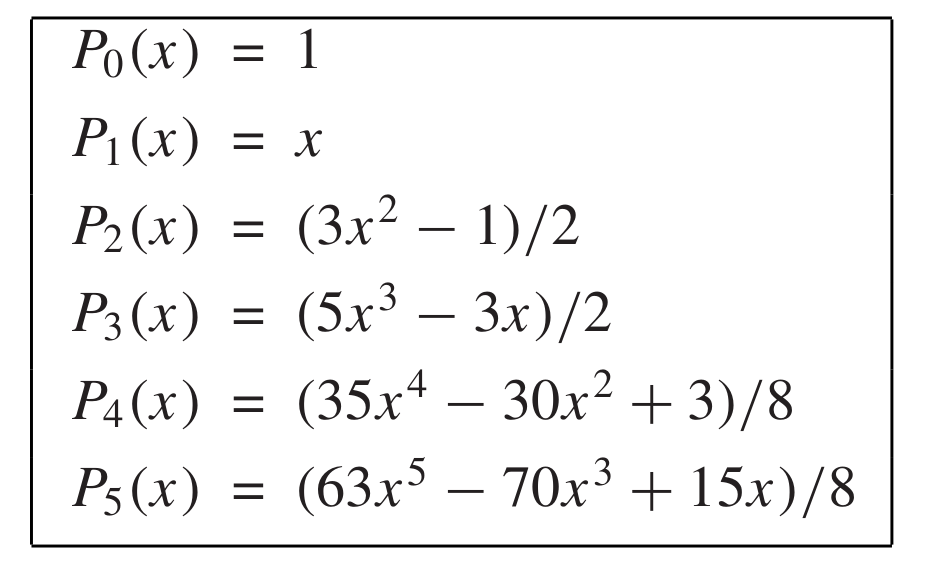
\includegraphics[width=0.4\linewidth]{legendre polynomials.png}\\~\\


\textbf{Table of Integrals}\\
$\ds \int\frac{a\sin(\theta)}{\sqrt{b+c\cos(\theta)}}d\theta=-\frac{2a\sqrt{b+c\cos(\theta)}}{c}+C$\\
$\ds \int\frac{1}{(a^2+x^2)^{3/2}}=\frac{x}{a^2\sqrt{a^2+x^2}}+C$\\
$\ds A\int\frac{\left(B+C\cos(\theta)\right)}{\left(D+E\cos(\theta)\right)^{\frac{3}{2}}}\sin(\theta)d\theta=-2A\frac{(E(C\cos(\theta)-B)+2CD)}{E^{2}\sqrt{E\cos(\theta)+D}}+\text{const}$\\
$\ds \int(a\cos^2(\theta)-b)\sin^2(\theta)\,d\theta=-\frac{a\sin(4\theta)-8b\sin(2\theta)+(16b-4a)\theta}{32}+C$\\
$\ds \int\frac{1}{\sqrt{s^2+z^2}}\,dz=\ln\left(\sqrt{z^{2}+s^{2}}+z\right)+C$
.\\~\\~\\



\textbf{Chapter 2 General Equations/Laws}\\
Generally, $\vec{\scripty{r}}=\vec{r}-\vec{r'}$, where $\vec{r}$ is a position of interest and $\vec{r'}$ is the position of some charge.\\
Force between two point charges $\ds\vec{F}=\frac{1}{4\pi\epsilon_0}\frac{qQ}{\scripty{r}^2}\hat{\scripty{r}}$\\~\\

\textit{Electric Field}\\
$\vec{F}=Q\vec{E}$\\
Electric field for $n$ point charges: $\ds\vec{E}(\vec{r})=\frac{1}{4\pi\epsilon_0}\sum_{i=1}^n\frac{q_i}{\scripty{r}_i^2}\hat{\scripty{r}}_i$\\
Electric field for continuous distributions:\\
$\ds\vec{E}(\vec{r})=\frac{1}{4\pi\epsilon_0}\int\frac{1}{\scripty{r}^2}\hat{\scripty{r}}\,dq$\\
$\ds\vec{E}(\vec{r})=\frac{1}{4\pi\epsilon_0}\int\frac{\lambda(\vec{r'})}{\scripty{r}^2}\hat{\scripty{r}}\,d\ell'$\\
$\ds\vec{E}(\vec{r})=\frac{1}{4\pi\epsilon_0}\int\frac{\sigma(\vec{r'})}{\scripty{r}^2}\hat{\scripty{r}}\,da'$\\
$\ds\vec{E}(\vec{r})=\frac{1}{4\pi\epsilon_0}\int\frac{\rho(\vec{r'})}{\scripty{r}^2}\hat{\scripty{r}}\,d\tau'$\\~\\

Superposition Principle: $\ds\vec{E}=\sum_{i=1}^n\vec{E}_i$\\
Gauss's Law:\\
$\ds\oint\vec{E}\cdot\vec{da}=\frac{q_{\text{enclosed}}}{\epsilon_0}$\\
$\ds\vec{\nabla}\cdot\vec{E}=\frac{\rho}{\epsilon_0}$\\
$\ds\oint\vec{E}\cdot\vec{d\ell}=0$\\
$\ds\vec{\nabla}\times\vec{E}=\vec{0}$\\~\\
\textit{Avg E}\\
$\ds\vec{E}_{\text{avg}}=\frac{1}{A_\mathcal{S}}\oint\displaylimits_{\text{S}}\vec{E}da$\\
$\ds\vec{E}_{\text{avg}}=\frac{1}{4\pi R^2}\oint\displaylimits_{\mathcal{S}}\vec{E}da$\\~\\

\textit{Electric Potential}\\
$\ds V(\vec{r})\equiv-\int_{\mathcal{O}}^{\vec{r}}\vec{E}\cdot \vec{d\ell}$\\
Potential Difference: $\ds V(\vec{b})-V(\vec{a})=-\int_{\vec{a}}^{\vec{b}}\vec{E}\cdot d\ell$\\
$\vec{E}=-\nabla V$\\
Superposition Principle: $\ds V=\sum_{i=1}^nV_i$\\~\\

Poisson's Equation: $\ds\nabla^2V=-\frac{\rho}{\epsilon_0}$\\
Laplace's Equation: $\ds\nabla^2V=0$\\~\\

Potentials from infinity\\
Point charge: $\ds V(\vec{r})=\frac{1}{4\pi\epsilon_0}\frac{q}{\scripty{r}}$\\
Continuous:\\
$\ds V(\vec{r})=\frac{1}{4\pi\epsilon_0}\int\frac{1}{\scripty{r}}dq$\\
$\ds V(\vec{r})=\frac{1}{4\pi\epsilon_0}\int\frac{\lambda(\vec{r'})}{\scripty{r}}d\ell'$\\
$\ds V(\vec{r})=\frac{1}{4\pi\epsilon_0}\int\frac{\sigma(\vec{r'})}{\scripty{r}}da'$\\
$\ds V(\vec{r})=\frac{1}{4\pi\epsilon_0}\int\frac{\rho(\vec{r'})}{\scripty{r}}d\tau'$\\~\\

Charge Distribution Boundary Conditions (where $\hat{n}$ is normal to charge surface)\\
$\ds\vec{E}_{\text{above}}-\vec{E}_{\text{below}}=\frac{\sigma}{\epsilon_0}\hat{n}$\\
$\ds V_{\text{above}}=V_{\text{below}}$\\
$\ds \frac{\partial V_{\text{above}}}{\partial n}-\frac{\partial V_{\text{below}}}{\partial n}=-\frac{1}{\epsilon_0}\sigma$\\~\\~\\

\textit{Work}\\
Work to move test charge: $\ds W=\int_{\vec{a}}^{\vec{b}}\vec{F}\cdot\vec{d\ell}=Q[V(\vec{b})-V(\vec{a})]$\\~\\
Work to assemble point charges\\
Add one more charge: $\ds W_i=\frac{1}{4\pi\epsilon_0}q_i\sum_{j\neq i}^n\frac{q_j}{\scripty{r}_{ij}}$\\
Assemble all charges: $\ds W_{\text{total}}=\frac{1}{4\pi\epsilon_0}\sum_{i=1}^n\sum_{j>i}^n\frac{q_iq_j}{\scripty{r}_{ij}}$\\
$\ds W=\frac{1}{2}\sum_{i=1}^nq_iV(\vec{r}_i)$\\~\\

Continuous Distribution\\
$\ds W=\frac{1}{2}\int\rho V\,d\tau$\\
$\ds W=\frac{\epsilon_0}{2}\left(\int\displaylimits_{\text{vol}}E^2\,d\tau+\oint\displaylimits_{\text{S}}V\vec{E}\cdot\vec{da}\right)$ (S encloses vol)\\
$\ds W=\frac{\epsilon_0}{2}\int E^2\,d\tau\ \ \ (\text{all space})$\\~\\~\\


\textbf{Conductor Facts }\\
$\vec{E}=\frac{\sigma}{\epsilon_0}\hat{n}$ (outside)\\
$\sigma=-\epsilon_0\frac{\partial V}{\partial n}$\\~\\~\\

\textbf{Capacitance}\\
$C=Q/V$, $Q=Q^+$ and $V=V^+-V^-=-\int_{(-)}^{(+)}\vec{E}\cdot\vec{d\ell}$.\\~\\~\\

\textbf{Chapter 3 General Equations}\\~\\

\textit{Method of Images}\\
$\ds W=\frac{1}{2}W_{\text{normal}}$\\~\\

\textit{Separation of Variables}\\
Cartesian:\\
$\ds X(x)=A^{kx}+Be^{-kx}$, $\ds Y(y)=C\sin(ky)+D\cos(ky)$\\
Spherical: (where $V(r,\theta)$)\\
$\ds V(r,\theta)=\sum_{\ell=0}^\infty\left(A_\ell r^\ell+\frac{B_\ell}{r^{\ell+1}}\right)P_\ell(\cos(\theta))$\\~\\

\textit{Multipole Expansion}\\
$\ds \frac{1}{\scripty{r}_\pm}\approx\frac{1}{r}(1\pm\frac{d}{2r}\cos(\theta))\ \ (\text{dipole})$\\
$\ds \frac{1}{\scripty{r}}=\frac{1}{r}\sum_{n=0}^\infty\left(\frac{r'}{r}\right)^nP_n(\cos(\alpha))$\\
$\ds V(\vec{r})=\frac{1}{4\pi\epsilon_0}\sum_{n=0}^\infty\frac{1}{r^{n+1}}\int(r')^nP_n(\cos(\alpha))\rho(\vec{r'})d\tau'$ (far away from $\rho$)\\
Dipole moment:\\
$\ds \vec{p}=q\vec{d}$\\
$\ds \vec{p}=\sum_iq_i\vec{r'}_i$\\
$\ds \vec{p}=\int\vec{r'}\rho(\vec{r'})\,d\tau'$\\
$\ds V_{\text{dip}}(\vec{r})=\frac{1}{4\pi\epsilon_0}\frac{\vec{p}\cdot\hat{r}}{r^2}$\\
Dipole Electric Field\\
$\ds \vec{E}_{\text{dip}}(r,\theta)=\frac{p}{4\pi\epsilon_0r^3}[2\cos(\theta)\hat{r}+\sin(\theta)\hat{\theta}]$\\
$\ds \vec{E}_{\text{dip}}(\vec{r})=\frac{1}{4\pi\epsilon_0}\frac{1}{r^3}[3(\vec{p}\cdot\hat{r})\hat{r}-\vec{p}]$\\~\\


\textbf{Chapter 4 General Equations}\\~\\

\textit{Induced Dipoles}\\
Atomic Polarizability $\alpha$: $\vec{p}=\alpha\vec{E}$\\
\textit{Polar Alignment}\\
Torque $\vec{N}=\vec{p}\times\vec{E}$\\
Force on dipole in field $\ds\vec{F}=(\vec{p}\cdot\vec{\nabla})\vec{E}$\\~\\

\textit{Polarization}\\
Polarization $\ds \vec{P}=\vec{p}/\text{vol}$\\
Surface Bound Charge: $\ds \sigma_b=\vec{P}\cdot\hat{n}$\\
Volume Bound Charge: $\ds \rho_b=-\vec{\nabla}\cdot\vec{P}$\\
$\ds V(\vec{r})=\frac{1}{4\pi\epsilon_0}\oint_\mathcal{S}\frac{\sigma_b}{\scripty{r}}da'+\frac{1}{4\pi\epsilon_0}\int_\mathcal{V}\frac{\rho_b}{\scripty{r}}d\tau'$\\~\\

\textit{Electric Displacement}\\
Electric Displacement: $\vec{D}=\epsilon_0\vec{E}+\vec{P}$\\
$\rho=\rho_b+\rho_\text{free}$\\
$\ds \vec{\nabla}\cdot\vec{D}=\rho_\text{free}$\\
or\\
$\ds \oint\vec{D}\cdot\vec{da}=Q_\text{free, enclosed}$\\
$\ds \vec{\nabla}\times\vec{D}=\vec{\nabla}\times\vec{P}$\\~\\

Boundary Conditions:\\
$\ds D^\perp_\text{above}-D^\perp_\text{below}=\sigma_f$\\
$\ds \vec{D}^\parallel_\text{above}-\vec{D}^\parallel_\text{below}=\vec{P}^\parallel_\text{above}-\vec{P}^\parallel_\text{below}$\\~\\

\textit{Linear Dielectrics}\\
Polarization $\vec{P}=\epsilon_0\chi_e\vec{E}$, where $\chi_e$ is electric susceptibility\\
Permitivity $\epsilon=\epsilon_0(1+\chi_e)=\epsilon_0\epsilon_r$\\
Relative Permitivity/Dielectric Constant: $\ds \epsilon_r=1+\chi_e=\frac{\epsilon}{\epsilon_0}$\\
$\vec{D}=\epsilon\vec{E}$\\
$\vec{P}=\epsilon_0(\epsilon_r-1)\vec{E}=\epsilon_0(\frac{\epsilon}{\epsilon_0}-1)\vec{E}$\\~\\

Homogeneous Linear Dielectric\\
$\vec{D}=\epsilon_0\vec{E}_\text{vac}$\\
$\ds \vec{E}=\frac{1}{\epsilon}\vec{D}=\frac{1}{\epsilon_r}\vec{E}_\text{vac}$\\~\\

Linear Dielectrics Boundaries\\
$\ds \epsilon_\text{above}\vec{E}_\text{above}-\epsilon_\text{below}\vec{E}_\text{below}=\sigma_f$\\
$\ds \epsilon_\text{above}\frac{\partial V_\text{above}}{\partial n}-\epsilon_\text{below}\frac{\partial V_\text{below}}{\partial n}=-\sigma_f$\\
$V_\text{above}=V_\text{below}$\\~\\

\textit{Dielectric Energy}\\
$\ds W=\frac{1}{2}CV^2$\\
$\ds C=\epsilon_rC_\text{vac}$\\
$\ds W=\frac{\epsilon_0}{2}\int\epsilon_rE^2\,d\tau=\frac{1}{2}\int\vec{D}\cdot\vec{E}\,d\tau$\\~\\


\textbf{Chapter 5 General Equations}\\~\\
\textit{Force on a test charge}\\
Lorentz Force Law: $\ds \vec{F}_\text{mag}=Q(\vec{v}\times\vec{B})$\\
E and B: $\ds \vec{F}=Q(\vec{E}+(\vec{v}\times\vec{B}))$\\
$W_\text{mag}=\int\vec{F}_\text{mag}\cdot\vec{d\ell}=0$\\~\\

\textit{Line Current}\\
$\vec{I}=\lambda\vec{v}$ or $I=\lambda v$\\
Force on wire: $\ds \vec{F}_\text{mag}=\int(\vec{v}\times\vec{B})\,dq=\int(\vec{v}\times\vec{B})\lambda\,d\ell=\int(\vec{I}\times\vec{B})\,d\ell=\int I(\vec{d\ell}\times\vec{B})$\\~\\

\textit{Surface Current}\\
Surface current density: $\ds\vec{K}=\frac{\vec{dI}}{d\ell_\perp}=\sigma\vec{v}$\\
where $d\ell_\perp$ is an infinitesimal width perpendicular to the current.\\
$\ds\vec{F}_\text{mag}=\int(\vec{v}\times\vec{B})\sigma\,da=\int(\vec{K}\times\vec{B})\,da$\\~\\

\textit{Volume Current}\\
Volume current density: $\ds\vec{J}=\frac{\vec{dI}}{da_\perp}=\rho\vec{v}$\\
where $da_\perp$ is an infinitesimal area perpendicular to the current.\\
$\ds\vec{F}_\text{mag}=\int(\vec{v}\times\vec{B})\rho\,d\tau=\int(\vec{J}\times\vec{B})\,d\tau$\\~\\

Total current crossing $\mathcal{S}$: $\ds I=\int_\mathcal{S}Jda_\perp=\int_\mathcal{S}\vec{J}\cdot\vec{da}_\perp$\\
Continuity equation: $\ds\vec{\nabla}\cdot\vec{J}=-\frac{\partial\rho}{\partial t}$\\~\\

Magnetostatics implications\\
$\ds\implies\frac{\partial\vec{J}}{\partial t}=\vec{0}$\\
$\ds\implies\vec{\nabla}\cdot\vec{J}=0$\\~\\

\textit{Biot-Savart Law:}\\
$\ds\vec{B}(\vec{r})=\frac{\mu_0}{4\pi}\int\frac{\vec{I}\times\hat{\scripty{r}}}{\scripty{r}^2}\,d\ell'=\frac{\mu_0}{4\pi}I\int\frac{\vec{d\ell}'\times\hat{\scripty{r}}}{\scripty{r}^2}$\\
$\ds\vec{B}(\vec{r})=\frac{\mu_0}{4\pi}\int\frac{\vec{K}(\vec{r'})\times\hat{\scripty{r}}}{\scripty{r}^2}\,da'$\\
$\ds\vec{B}(\vec{r})=\frac{\mu_0}{4\pi}\int\frac{\vec{J}(\vec{r'})\times\hat{\scripty{r}}}{\scripty{r}^2}\,d\tau'$\\~\\

$\ds\vec{\nabla}\cdot\vec{B}=0$\\
Ampere's Law: $\ds\vec{\nabla}\times\vec{B}=\mu_0\vec{J}$\\
Ampere's Law: $\ds\oint\vec{B}\cdot\vec{d\ell}=\mu_0I_\text{enc}$\\~\\

\textit{Magnetic Vector Potential:}\\
Definition: $\ds\vec{B}=\vec{\nabla}\times\vec{A}$\\
$\ds\vec{\nabla}\cdot\vec{A}=0$\\
$\ds\nabla^2\vec{A}=-\mu_0\vec{J}$\\~\\

Non-infinite current case:\\
$\ds\vec{A}(\vec{r})=\frac{\mu_0}{4\pi}\int\frac{\vec{J}(\vec{r'})}{\scripty{r}}d\tau'$\\
$\ds\vec{A}(\vec{r})=\frac{\mu_0}{4\pi}\int\frac{\vec{K}(\vec{r'})}{\scripty{r}}da'$\\
$\ds\vec{A}(\vec{r})=\frac{\mu_0}{4\pi}\int\frac{\vec{I}(\vec{r'})}{\scripty{r}}d\ell'=\frac{\mu_0I}{4\pi}\int\frac{1}{\scripty{r}}\vec{d\ell'}$\\~\\

\textit{Boundary Conditions}\\
$\ds B_\text{above}^\perp=B_\text{below}^\perp$\\
$\ds B_\text{above}^\parallel-B_\text{below}^\parallel=\mu_0K$\\
$\ds \vec{B}_\text{above}-\vec{B}_\text{below}=\mu_0(\vec{K}\times\hat{n})$\\
$\ds \vec{A}_\text{above}=\vec{A}_\text{below}$\\
$\ds \oint\vec{A}\cdot\vec{d\ell}=\int\vec{B}\cdot\vec{da}=\Phi$\\
$\ds \frac{\partial\vec{A}_\text{above}}{\partial n}-\frac{\partial\vec{A}_\text{below}}{\partial n}=-\mu_0\vec{K}$\\~\\

\textit{Multipole Expansion}\\
$\ds\vec{A}(\vec{r})=\frac{\mu_0I}{4\pi}\oint\frac{1}{\scripty{r}}\vec{d\ell'}=\frac{\mu_0I}{4\pi}\sum_{n=0}^\infty\frac{1}{r^{n+1}}\oint(r')^nP_n(\cos(\alpha))\vec{d\ell'}$\\
$\ds\vec{A}(\vec{r})=\frac{\mu_0I}{4\pi}\left[\frac{1}{r}\oint\vec{d\ell'}+\frac{1}{r^2}\oint r'\cos(\alpha)\,\vec{d\ell'}+\frac{1}{r^3}\oint(r')^2\left(\frac{3}{2}\cos^2(\alpha)-\frac{1}{2}\right)\vec{d\ell'}+\dots\right]$\\
Volume Current: $\ds\vec{A}(\vec{r})=\frac{\mu_0}{4\pi}\sum_{n=0}^\infty\frac{1}{r^{n+1}}\oint(r')^nP_n(\cos(\alpha))\vec{J}d\tau$\\
$\ds \vec{A}_\text{dip}(\vec{r})=\frac{\mu_0}{4\pi}\frac{\vec{m}\times\hat{r}}{r^2}$\\
where magnetic dipole moment $\vec{m}=I\int\vec{da}=I\vec{a}$\\
Vector area: $\vec{a}=\frac{1}{2}\oint\vec{r}\times\vec{d\ell}$\\
Pure Magnetic Dipole\\
$\ds \vec{A}_\text{dip}=\frac{\mu_0}{4\pi}\frac{m\sin(\theta)}{r^2}\hat{\phi}$\\
$\ds \vec{B}_\text{dip}=\vec{\nabla}\times\vec{A}_\text{dip}=\frac{\mu_0m}{4\pi r^3}(2\cos(\theta)\hat{r}+\sin(\theta)\hat{\theta})$\\
$\ds\vec{B}_\text{dip}(\vec{r})=\frac{\mu_0}{4\pi}\frac{1}{r^3}\left[3(\vec{m}\cdot\hat{r})\hat{r}-\vec{m}\right]$\\~\\

\textbf{Chapter 6 General Equations}\\
Torque on magnetic dipole: $\ds \vec{N}=\vec{m}\times\vec{B}$.\\


.\\~\\


\textbf{Specific Examples}\\
\textit{Infinite Plane of Charge}\\
$\ds \vec{E}=\frac{\sigma}{2\epsilon_0}\hat{r}$\\~\\

\textit{Two Infinite Planes of Opposite Charge}\\
$\ds \vec{E}=\frac{\sigma}{\epsilon_0}\hat{r}$ (from positive to negative, between the planes)\\
$\ds \vec{E}=\vec{0}$ otherwise\\
$\ds C=A\epsilon_0/d$\\~\\

\textit{Charged Spherical Shell}\\
$\ds \vec{E}=\frac{1}{4\pi\epsilon_0}\frac{q}{r^2}\hat{r}$ (outside)\\
$\ds \vec{E}=\vec{0}$ (inside)\\
$\ds V(r)=\frac{1}{4\pi\epsilon_0}\frac{q}{r}$ (outside)\\
$\ds V(r)=\frac{1}{4\pi\epsilon_0}\frac{q}{R}$ (inside)\\~\\

\textit{Conducting Sphere with Grounded Surface and External Point Charge}\\
Outer charge $q$ distance: $a$\\
Inner charge: $q'=-\frac{R}{a}q$ at distance $b=\frac{R^2}{a}$.\\~\\

\textit{Uncharged Metal Sphere in Uniform Electric Field}\\
$\ds V(r,\theta)=-E_0\left(r-\frac{R^3}{r^2}\right)\cos(\theta)$ (relative to xy plane)\\~\\

\textit{Spherical Shell of Varying Charge Density}\\
$\ds V(r,\theta)_\text{inside}=\sum_{\ell=0}^\infty A_\ell r^\ell P_\ell(\cos(\theta))$\\
$\ds V(r,\theta)_\text{outside}=\sum_{\ell=0}^\infty\frac{B_\ell}{r^{\ell+1}}P_\ell(\cos(\theta))$\\
where\\
$\ds B_\ell=A_\ell R^{2\ell+1}$\\
$\ds A_\ell=\frac{1}{2\epsilon_0R^{\ell-1}}\int_0^\pi\sigma_0(\theta)P_\ell(\cos(\theta))\sin(\theta)\,d\theta$\\
if $\sigma_0(\theta)=P\cos(\theta)$, then\\
$\ds V(r,\theta)=\begin{cases}
        \ds \frac{P}{3\epsilon_0}r\cos(\theta), & r\leq R\\
        \ds \frac{P}{3\epsilon_0}\frac{R^3}{r^2}\cos(\theta), & r\geq R\\
    \end{cases}$\\~\\

\textit{Sphere of Homogeneous Linear Dielectric Material in Uniform Field}\\
$\ds \vec{E}_\text{inside}=\frac{3}{\epsilon_r+2}\vec{E}_0$\\~\\

\textit{Cyclotron Motion}\\
$\ds QvB=m\frac{v^2}{R}$\\
or momentum $p=QBR$\\~\\

\textit{Infinite Line of Current}\\
Magnetic field from $\theta_1$ to $\theta_2$: $\ds B(\theta_1,\theta_2)=\frac{\mu_0I}{4\pi s}\int_{\theta_1}^{\theta_2}\cos(\theta)\,d\theta=\frac{\mu_0I}{4\pi s}[\sin(\theta_2)-\sin(\theta_1)]$\\
Magnetic Field from whole wire: $\ds\vec{B}=\frac{\mu_0I}{2\pi s}\hat{\phi}$\\~\\

\textit{Loop of Current}\\
Magnetic field above center: $\ds B(z)=\frac{\mu_0I}{2}\frac{R^2}{(R^2+z^2)^{3/2}}$\\~\\

\textit{Solenoid}\\
Magnetic field on central axis: $\ds B(\theta_1,\theta_2)=\frac{\mu_0nI}{2}[\cos(\theta_2)-\cos(\theta_1)]$\\
Infinite Solenoid: $\ds B=\mu_0nI$\\~\\

\textit{Toroidal Coil}\\
$\ds\vec{B}=\begin{cases}
    \ds\frac{\mu_0NI}{2\pi s}\hat{\phi} & (\text{inside coil})\\
    \vec{0} & (\text{outside coil})\\
\end{cases}$



.\\~\\

\textbf{Other Physics Topics}\\
Momentum: $\vec{p}=m\vec{v}$\\
Conservation of Momentum: $\vec{p}=m\vec{v}=\text{const}$\\
Kinetic Energy: $K=\frac{1}{2}mv^2$\\
Total Energy: $E=K+U$\\
Conservation of Energy: $E=K+U=\text{const}$\\~\\

Uniform Circular Motion Force: $\ds \vec{F}=-m\frac{v^2}{r}\hat{r}$\\~\\


\textbf{Helpful Specific Integrals}\\
$\ds \frac{2\pi R^2\sigma}{4\pi\epsilon_0}\int_0^{\pi}\frac{(z-R\cos(\theta))\sin(\theta)\,d\theta}{(R^2+z^2-2Rz\cos(\theta))^{3/2}}\hat{z}=\frac{2\pi R^2\sigma}{4\pi\epsilon_0}\frac{1}{z^2}\left(\frac{z+R}{\sqrt{z^2+2Rz+R^2}}+\frac{z-R}{\sqrt{z^2-2Rz+R^2}}\right)\hat{z}$\\~\\~\\


\textbf{Units}\\
Coulomb: C\\
Volt: V$=$N/C\\
Farad: F$=$C/V\\
Ampere: A$=$C/s\\
Tesla: T$=$N/(A m)\\



\newpage





    

    











\end{flushleft}

\end{document}
